In this chapter we shall build our approach to user modeling.
We will first explain the reasoning behind our hypotheses,
before developing an approach to adaptive aggregation,
called \emph{stacked user modeling}.
We will then show how to use these \emph{meta models}
to perform prediction aggregation in a recommendation scenario,
and rank aggregation in an information retrieval scenario.
The performance of our method will be tested in the next chapter.

\section{Latent Subjectivity}
\label{sec:reasoning}

As described in the previous chapter, 
there are many ways of predicting the
relevance of an item to a user. 
In fact, judging by the number of different approaches,
the only limiting factor seems to be the different 
patterns researchers discover in available data.

As described in Section \ref{sec:aggregate},
modern approaches to recommender systems try to combine many of these methods.
By leveraging so called \emph{disjoint patterns}
in the data, several less than optimal predictors
can be combined, so that the combination outperforms the individual algorithms.
Moderns search engines work much in the same way,
combining multiple ranking signals into a final results list
(see Section \ref{subsec:signals}).

Why then, when we have all these valid approaches, would we need yet another technique?
As explained in Chapter \ref{chap:intro}, 
we believe the \emph{latent subjectivity problem}
is a fundamental issue with each approach described so far.
Consider the following examples of relevance judgement:

\begin{itemize*}
  \item PageRank \citep{Bender2005} assumes that the relevance of a web page is 
  represented by its authority, as computed from inbound links from other sites.
  \item Some systems considers a user's social connections to be important
  in ranking search results, when performing personalized search (e.g. \cite{Carmel2009}).
  \item When recommending movies, one predictor may be based on the ratings
  of users with similar profile details. Another predictor might be 
  dependent on some feature, e.g. production year of well liked movies.
  \item SVD-based approaches assume global patterns and groups of users and items
  are best suited to produce predictions (see Section \ref{subsec:recommender:examples}).
  \item Recommendations based on the Pearson Correlation Coefficient \cite[p.11]{Segaran2007}
  assumes that the statistical correlation between user ratings is a good
  measure for user similarity.
\end{itemize*}

While these methods may perform well, their selection
reflects how whoever created the system assumes how users
can and \emph{should} be modeled. This underlying subjectivity is not desirable.
We see two different approaches one can take when creating a recommender system,
represented by two questions:

\clearpage

\begin{enumerate*}
  \item What combination of which methods will accurately predict unknown scores?
  \item Which methods could possibly help predict a score for a user or an item?
\end{enumerate*}

The first question is what has to be considered in traditional modeling aggregation.
First, a set of applicable methods leveraging disjoint patterns must be selected. 
Then, an optimal and generalized combination of these must be found,
most often through minimizing the average error across all users.

The second question is quite different. 
Instead of looking for an optimal set of methods and an optimal combination,
we look for the set of \emph{any applicable methods} that \emph{some users} might find helpful,
or that might work for \emph{some items}.
We believe this is a much simpler problem. 
Instead of trying to generalize individuality,
it can be embraced, by allowing users to implicitly and automatically select which methods they prefer,
from a large set of possible predictors.

As explained in Chapter \ref{chap:intro}, 
assuming that users will place similar importance on each modeling method is 
contrary to the goals of user modeling. 
Our goal should instead be a system which can leverage the differences
between users and employ the available algorithms based on their individual preferences.

Just as users are different, items have their own characteristics.
Needless to say, items are often quite different from another,
along a myriad of dimensions. For example,
if items correspond to websites, the number of metrics we can use to judge
the relevance of an item is immense.
If items are indeed as different as the users themselves, it stands to reason that the same 
modeling method will not perform as well for every item.

An approach where we only need to consider the second question is desirable.
Regardless, both traditional, single-approach modeling methods, and modern aggregation approaches
often treat every user and item the same. No matter its intrinsic qualities, an element will be judged
by the same methods as every other element. 

This chapter will develop a way to aggregate a host of modeling methods on a per-user and per-item basis.
By adapting the aggregation to the current item and user, we should be able to mitigate the latent subjectivity problem. 
This adaptive aggregation is performed implicitly and automatically,
without any extra interaction required from each user.

As mentioned in Chapter \ref{chap:intro}, this has an important consequence.
If each algorithm is \emph{only used} in situations it will probably perform well,
any possible recommender algorithm becomes a worthy addition.
In other words, instead of finding an optimal combination,
we can use any algorithm that \emph{might work for some elements}
in our aggregation.

With adaptive recommenders, the users are in control of which methods best fit their needs, and
a method's priority is influenced by how well it performs for the current item.
However, in order to test whether or not these assumptions hold,
we need a set of testable hypotheses.

\clearpage

\section{Hypotheses}

So far we have taken a look at approaches to recommendations and personalized search:
Traditionally, a single method that considers some pattern in the data is used.
Modern techniques blend different methods to achieve a combined accuracy 
that outranks the performance of each individual method.

However, based on the notion of latent subjectivity in method selection and aggregation,
we desire an even more personalized technique. 
To this end, this paper will test three hypotheses (H1-H3), in an effort to establish
whether per-user aggregation is a viable technique. First:

{
  \itshape
  $\mathbf{H1}$: The accuracy of user-item relevance predictions can be improved
  by blending multiple modeling methods on a per-user basis:
  $\forall m \in M: \mathrm{error}(am_u) < \mathrm{error}(m)$.
}

It stands to reason that if a recommender system is indeed impaired
by the subjective selections of modeling methods,
a per-user blend of these methods should outperform each of the individual approaches.
Second:

{
  \itshape
  $\mathbf{H2}$: A per-user aggregation method can outperform global and generalized 
  blending methods:
  $\forall a \in A: \mathrm{errorr}(am_u) < \mathrm{error}(a)$.
}

If our assumption that model aggregation inherits the subjective nature of its chosen parts,
a per-user aggregation without such misplaced subjectivity should outperform a
generalized blending.
Third:

{
  \itshape
  $\mathbf{H3}$: The result set from an information retrieval query
  can be personalized by blending multiple modeling methods on a per-user basis.
}

As described in Section \ref{subsec:signals},
every measure that influence the final ranking of results from a search engine
can be seen as individual signals. Each signal, be it an IR score,
something like PageRank or the result of a user modeling method,
contributes to the final ranking.
As the aggregation of these signals are the same problem faced
when aggregating recommender systems,
a per-user approach to blending signals should be able to
produce a set of personalized search results.
In other words, techniques from information retrieval and user modeling
should be combined on a per-user basis to provide individually adapted results.


\section{Adaptive Recommenders}
\label{sec:usermetamodeling}

\emph{Adaptive Recommenders} (AR) is a technique for combining many recommender systems
in a way that is optimal for the each user and each item.
Given that we wish to predict the relevance of an item to a user,
using many methods that consider disjoint data patterns,
we have two important questions:

\begin{enumerate*}
  \item What rating does each method predict?
  \item How accurate will each of these predictions be?
\end{enumerate*}

Recommender systems traditionally only care about the first question:
a single method is used to predict an unknown rating.
Modern aggregation techniques goes one step further, and combines many methods using a generic (often weighted) combination.
We wish to make the aggregation \emph{adaptive},
so that the aggregation itself depends on which user and which item we are considering.

Formally, we define adaptive recommenders as \emph{adapting a set of recommender systems
with another complementary set of recommender systems} 
(see Figure \ref{fig:adaptiveusermodeling}).
This then is a form of meta-modeling, where one set of modeling methods is adapted by another set of modeling methods.
The first set creates standard prediction scores, and answers the first question.
The second set predicts how accurate each method will be for the current user and item,
answering the second question.
The interesting bit is that AR can use recommender systems for both these tasks, as we shall see.
A system for adaptive recommenders is specified by a 6-tuple:

\begin{eqnarray*}
  \mathrm{AR} &=& (Items, Users, Ratings, Framework, Methods, Adapters)\\
              &=& (I,U,R,F,M,A).
\end{eqnarray*}
%
We have sets of $Users$ and $Items$, and a set of $Ratings$.
Each user $u \in U$ can produce a rating $r \in R$ of an item $i \in I$.
As mentioned, items can be just about anything, for example documents, websites, movies, events, or indeed, other users.
The ratings can be explicitly provided by users, for example by rating movies,
or they can be mined from existing data, for example by mining query logs.
As before, we use the term \emph{rating} loosely --- equivalent terms include \emph{relevance}, \emph{utility},
\emph{score} or \emph{connection strength}. In other words, this is a measure of what a user thinks of an item
in the current domain language. However, since \emph{rating} will match the case study we present in the next chapter,
we will be using this term. 

\begin{figure}[t]
  \centering 
  \begin{minipage}{0.49\textwidth}
    \centering 

    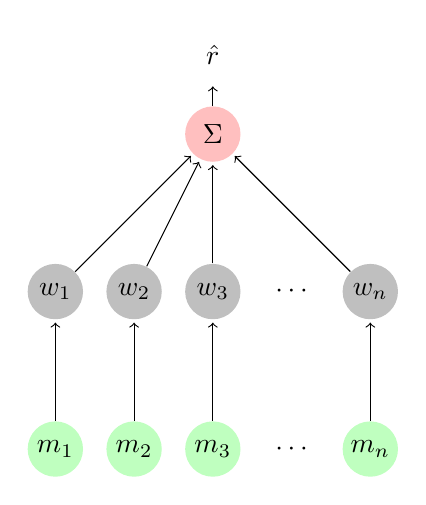
\begin{tikzpicture}[shorten >=1pt,->,draw=black, node distance=\layersep]
      \tikzstyle{every pin edge}=[<-,shorten <=2pt]
      \tikzstyle{node}=[circle,fill=black!25,minimum size=20pt,inner sep=0pt];
      \tikzstyle{method}=[node,fill=green!25];
      \tikzstyle{weight}=[node,fill=black!25];
      \tikzstyle{error}=[node,fill=blue!25];
      \tikzstyle{agg}=[node,fill=red!25];
      \tikzstyle{txt}=[node,fill=white];
       
      \node[method] (M1) at (0,-6) {$m_1$};      
      \node[method] (M2) at (1,-6) {$m_2$};         
      \node[method] (M3) at (2,-6) {$m_3$};         
      \node[txt]    (MS) at (3,-6) {$\cdots$}; 
      \node[method] (MN) at (4,-6) {$m_n$};
      \node[weight] (W1) at (0,-4) {$w_1$};      
      \node[weight] (W2) at (1,-4) {$w_2$};         
      \node[weight] (W3) at (2,-4) {$w_3$};         
      \node[txt]    (WS) at (3,-4) {$\cdots$}; 
      \node[weight] (WN) at (4,-4) {$w_n$};
      \node[agg]    (AG) at (2,-2) {$\Sigma$};
      \node[txt]    (RS) at (2,-1)  {$\hat{r}$};
      
      \path (M1) edge (W1);
      \path (M2) edge (W2);
      \path (M3) edge (W3);
      \path (MN) edge (WN);
      \path (W1) edge (AG);
      \path (W2) edge (AG);
      \path (W3) edge (AG);
      \path (WN) edge (AG);
      \path (AG) edge (RS);
    \end{tikzpicture}
  \end{minipage} 
  \hfill 
  \begin{minipage}{0.49\textwidth}
    \centering 

    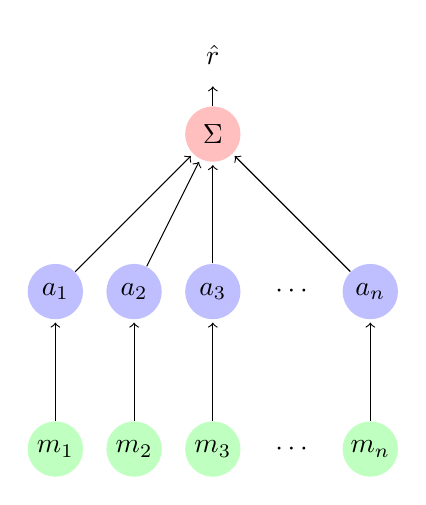
\begin{tikzpicture}[shorten >=1pt,->,draw=black, node distance=\layersep]
      \tikzstyle{every pin edge}=[<-,shorten <=2pt]
      \tikzstyle{node}=[circle,fill=black!25,minimum size=20pt,inner sep=0pt];
      \tikzstyle{method}=[node,fill=green!25];
      \tikzstyle{weight}=[node,fill=black!25];
      \tikzstyle{error}=[node,fill=blue!25];
      \tikzstyle{agg}=[node,fill=red!25];
      \tikzstyle{txt}=[node,fill=white];
       
      \node[method] (M1) at (0,-6) {$m_1$};      
      \node[method] (M2) at (1,-6) {$m_2$};         
      \node[method] (M3) at (2,-6) {$m_3$};         
      \node[txt]    (MS) at (3,-6) {$\cdots$}; 
      \node[method] (MN) at (4,-6) {$m_n$};
      \node[error]  (E1) at (0,-4) {$a_1$};      
      \node[error]  (E2) at (1,-4) {$a_2$};         
      \node[error]  (E3) at (2,-4) {$a_3$};         
      \node[txt]    (ES) at (3,-4) {$\cdots$}; 
      \node[error]  (EN) at (4,-4) {$a_n$};
      \node[agg]    (AG) at (2,-2) {$\Sigma$};
      \node[txt]    (RS) at (2,-1)  {$\hat{r}$};
      
      \path (M1) edge (E1);
      \path (M2) edge (E2);
      \path (M3) edge (E3);
      \path (MN) edge (EN);
      \path (E1) edge (AG);
      \path (E2) edge (AG);
      \path (E3) edge (AG);
      \path (EN) edge (AG);
      \path (AG) edge (RS);
    \end{tikzpicture}
  \end{minipage} 
  \vspace{2em}
  \caption[Comparison of Aggregation and Adaption]{
    Comparison of aggregation and adaption:
    (left) modern aggregation approaches uses a set of pretrained weights
    to prioritize each modeling method.
    The weighted predictions are aggregated into a final prediction $\hat{r}$.
    (right) Adaptive user modeling employs secondary modeling methods instead
    of weights. These estimate the accuracy of the initial method
    for the current user and item.
  }
  \label{fig:layer:comparison}
\end{figure}




The $Framework$ variable specifies how the data is represented.
The two canonical ways of representing users, items and ratings are graphs and matrices (see Section \ref{sec:recommender}).
We shall use a matrix, where the first dimension corresponds to users, the second to items, and each populated cell is an explicit or implicit rating:

\begin{eqsp}
 R_{u,i} =
 \begin{pmatrix}
  r_{1,1} & r_{1,2} & \cdots & r_{1,i} \\
  r_{2,1} & r_{2,2} & \cdots & r_{2,i} \\
  \vdots  & \vdots  & \ddots & \vdots  \\
  r_{u,1} & r_{u,2} & \cdots & r_{u,i}
 \end{pmatrix}.
\end{eqsp}
%
As we wish to leverage disjoint data patterns, we have a set of modeling $Methods$, 
each with their own way of estimating unknown ratings. 
Each model $m \in M$ is used to compute independent and hopefully complimentary predictions.
In our case, these methods are recommender systems.

As demonstrated in Chapter \ref{chap:theory}, there are many different recommendation algorithms,
that consider different aspects in the data, for example users, items and ratings, as well as 
sources such as intra-user connections in social networks or intra-item connections in information retrieval systems.
Examples of such recommender systems include Slope One predictions, SVD factorization and Nearest Neighbor weighted predictions
(see Section \ref{subsec:recommender:examples}).
These methods predict unknown connections between users and items based on some pattern in the data,
for example user profile similarity, rating correlations or social connections.
As previously explained, to achieve the best possible combined result, we wish to use methods that look at disjoint patterns, 
i.e. complementary predictive parts of the data (see Section \ref{sec:aggregate}).

The $Adapters$ part of our 6-tuple refers to the second level of user modeling methods.
In traditional prediction aggregation this is a simple linear function for combining the different predictions,
for example by pre-computing a set of weights, one for each method.
As found by \citet[p6]{Bell2007} the accuracy of the combined predictor is more dependent on the 
ability of the various predictors to expose different aspects of the data, than on 
the individual accuracy of each predictor.
As described in Section \ref{sec:aggregate}, multiple prediction results are normally 
combined into a final singular result,
based on a generalized combination found by minimizing some error across all users.

With adaptive recommenders, the $Adapters$ are themselves user modeling methods 
(see Figure \ref{fig:layer:comparison}).
However, instead of modeling users, we wish to model each recommender system.
More specifically, we wish to model the \emph{accuracy} of each recommender system.
Methods in this second layer are used to predict how accurate each of their corresponding basic recommenders will be.
It is these methods that will allow us to do adaptive aggregation based on the current user and item.
We then have two distinct layers of user modeling 
(see Figure \ref{fig:adaptiveusermodeling}):

\begin{figure}
  \center
  \def\layersep{1.8cm}
  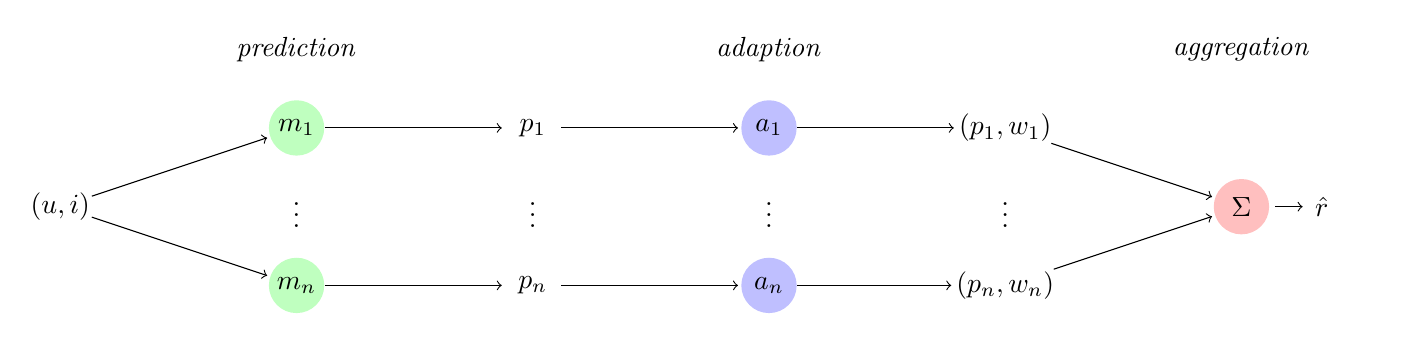
\begin{tikzpicture}[shorten >=1pt,->,draw=black, node distance=\layersep]

    \tikzstyle{every pin edge}=[<-,shorten <=2pt]
    \tikzstyle{node}=[circle,fill=black!25,minimum size=20pt,inner sep=0pt]
    \tikzstyle{input node}=[node, fill=green!25];
    \tikzstyle{output node}=[node, fill=red!25];
    \tikzstyle{hidden node}=[node, fill=blue!25];
    \tikzstyle{annot} = [text width=10em, text centered]
    \tikzstyle{txt}=[node,fill=white];
    
    \node[txt] (UI) at (0,-2) {$(u,i)$};  

    \node[input node] (I-1) at (\layersep,-1) {$m_1$};
    \node[txt]        (I-D) at (\layersep,-2) {$\vdots$};
    \node[input node] (I-N) at (\layersep,-3) {$m_n$};
    
    \node[txt] (P-1) at (\layersep*2, -1) {$p_1$};
    \node[txt] (P-D) at (\layersep*2, -2) {$\vdots$};
    \node[txt] (P-N) at (\layersep*2, -3) {$p_n$};

    \node[hidden node] (H-1) at (\layersep*3, -1) {$a_1$};    
    \node[txt]         (H-D) at (\layersep*3, -2) {$\vdots$};    
    \node[hidden node] (H-N) at (\layersep*3, -3) {$a_n$};    

    \node[txt] (R-1) at (\layersep*4, -1) {$(p_1,w_1)$};
    \node[txt] (R-D) at (\layersep*4, -2) {$\vdots$};
    \node[txt] (R-N) at (\layersep*4, -3) {$(p_n,w_n)$};
    
    % hidden helper node
    \node[txt] (HH)  at (\layersep*5,-1) {};

    % Draw the output layer node
    \node[output node,pin={[pin edge={->}]right:$\hat{r}$}] at (\layersep*5,-2) (O) {$\Sigma$};
    
    \path (UI) edge (I-1);
    \path (UI) edge (I-N);

    \path (I-1) edge (P-1);
    \path (I-N) edge (P-N);

    \path (P-1) edge (H-1);
    \path (P-N) edge (H-N);

    \path (H-1) edge (R-1);
    \path (H-N) edge (R-N);

    \path (R-1) edge (O);
    \path (R-N) edge (O);

    % Annotate the layers
    \node[annot,above of=I-1, node distance=1cm] {\emph{prediction}};
    \node[annot,above of=H-1, node distance=1cm] {\emph{adaption}};
    \node[annot,above of=HH,  node distance=1cm] {\emph{aggregation}};
  \end{tikzpicture}

  \vspace{1em}
  \caption[The Layers of Recommenders]{
    Layers of recommenders. 
  }
  \label{fig:adaptiveusermodeling}
\end{figure}


\begin{enumerate}
  \item
    \emph{The methods layer} consists of traditional user modeling methods, that use a single aspect of the data to produce predictions.
    When presented with an item and a user, these methods produce a predicted rating $\hat{r}_{u,i}$ based on their algorithms.
  \item
    \emph{The adaptive layer} is another set of corresponding modeling methods, that work a bit differently.
    These methods take an item and a user and estimates how well its underlying method will perform this prediction.
    The accuracy estimations are then combined with the predictions by aggregation.
    Each of these adaptive methods do not have to employ the same algorithm as their corresponding methods,
    the layers are only similar in that both consist of recommender systems.
\end{enumerate}

Another way of describing (and implementing) these two levels is through 
the $\mathrm{map}$ and $\mathrm{reduce}$ functions of functional programming.
For example, we can express prediction aggregation as 

\begin{eqsp}
  \hat{r}_{u,i} = \mathrm{reduce}(u, i, \mathrm{map}(M, u, i)).
\end{eqsp}
%
First, each modeling method is applied by the $\mathrm{map}$ function, with the current user, item and set of modeling methods as input.
This operation returns a set of scalar prediction values. 
These values are then combined by the $\mathrm{reduce}$ function, which also takes the current user and item as input.
In our terms, $\mathrm{map}$ is the methods layer, and $\mathrm{reduce}$ is the adaptive layer.
If we wish to do rank aggregation, the equation is a bit different:

\begin{eqsp}
  \tau_{u,n} = \mathrm{reduce}(u, \mathrm{map}(M,u,n)).
\end{eqsp}
%
Here, $\tau_{u}$ is the list of recommended items for user $u$ (following the notation in \citet[p3]{Dwork2001}).
Note that there is no input item in this formula as we wish to produce a ranking of the top $n$ recommended items.
The result is an adaptively sorted list of the top $n$ items for the current user.
A common use case for rank aggregation is personalized search:
an IR algorithm restricts the item space, which is then adapted by recommender systems,
as we shall see.

Expressing ourselves in terms of $\mathrm{map}$ and $\mathrm{reduce}$ is helpful 
as this will guide our implementation.
Note that our terminology is a bit different from the proper MapReduce framework
for parallel computation (as explained in \citet[p75]{Manning2008}).
However, as with the standard key/value approach to MapReduce,
the fact that our tasks can be run in parallel will help
us implement efficient algorithms.


\subsection{Adaptive Aggregation}

To perform adaptive recommender aggregation, we need the $Adapters$ to be actual recommender systems.
Until now we have talked about both prediction aggregation (scores) and rank aggregation (sorted lists).
For now we shall stick to scalar predictions, but will return to rank aggregation in Section \ref{sec:methods:rank}.

The simplest generalized way of prediction aggregation is to take the average of all predictions made
by the different methods (e.g. \citet[p3]{Aslam2001}):

\begin{eqsp}
  \hat{r}_{u,i} = \frac{1}{N} \sum_{m \in M} p(m,u,i).
\end{eqsp}
%
Here, $\hat{r}_{u,i}$ is the estimated rating from user $u$ to item $i$,
$N$ is the number of methods in $M$, and $p(m,u,i)$ is the predicted rating from method $m$.
To achieve an even more optimal result, 
many aggregators weigh each method differently (e.g. \cite{Claypool1999}):

\begin{eqsp}
  \hat{r}_{u,i} = \sum_{m \in M} w_{m} \times p(m,u,i) 
  \quad \text{where} \quad 0 \leq w_{m} \leq 1, \quad \sum_{m \in M} (w_m) = 1.
\end{eqsp}
%
In this equation, $w_m$ is the weight applied to modeling method $m$. 
These weights fall in the range $[0,1]$ and sum up to $1$.
As described in \ref{sec:aggregate}, 
these weights can be estimated by different machine learning methods.
However, as discussed in Section \ref{sec:reasoning},
this is still a generalized result, averaged across every user and item.
The system assumes that the best average result is the best result for each individual user and item.
This means that, even with method-specific weights, we are still hindered by the latent subjectivity problem.

In order to leverage as many patterns as possible while sidestepping any latent subjectivity,
we need \emph{adaptive weights} that are computed specifically for each combination of a user and an item.
This is more difficult than simply estimating generalized weights.
If we wish each weight to be combination-specific, then pre-computing each weight for each method becomes unfeasible.
We would have to compute a weight for each method for each possible rating.
The adaptive weights also have to be estimated just as the unknown ratings:

\begin{eqsp}
  \hat{r}_{u,i} = \sum_{m \in M} p_{w}(m,u,i) \times p_{r}(m,u,i)
  \quad \text{where} \quad
  \sum_{m \in M} (p_{w}(m,u,i)) = 1.
\end{eqsp}
%
Here, $p_w(m,u,i)$ is the predicted optimal weight for method $m$ when applied to user $u$ and item $i$.
Adaptive recommenders is one way to estimating these weights, i.e. one way to implement $p_w$.

We wish to use standard recommender systems for predicting optimal adaptive weights.
To do this, we need to create a matrix (or graph)
that stores known values of how accurate some of the rating predictions will be.

The key insight is that \emph{the predicted accuracy of a method is the opposite of its predicted error}.
By modeling the errors of a method through standard recommender systems,
we can in turn predict errors for untested combinations
(see Figure \ref{fig:adaptiveweights}).
If we predict the error of a recommender system for a user and an item,
we have also predicted its accuracy.
To achieve this, we create an \emph{error matrix}:

\begin{figure}[t]
  \center
  \def\layersep{3cm}
  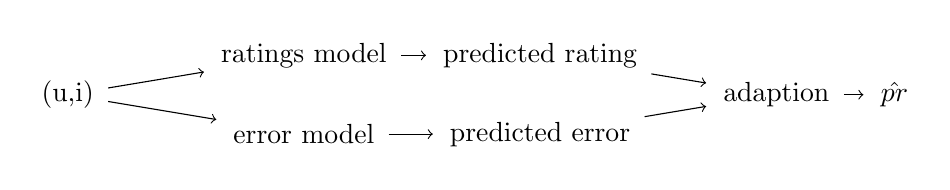
\begin{tikzpicture}[shorten >=1pt,->,draw=black, node distance=\layersep]

    \tikzstyle{every pin edge}=[<-,shorten <=2pt]
    \tikzstyle{rmodel}=[rectangle,fill=green!25,minimum size=20pt,inner sep=5pt]
    \tikzstyle{emodel}=[rectangle,fill=blue!25,minimum size=20pt,inner sep=5pt]
    \tikzstyle{amodel}=[rectangle,fill=red!25,minimum size=20pt,inner sep=5pt]
    \tikzstyle{blank}=[rectangle,fill=white,minimum size=20pt,inner sep=5pt]
    
    \node[blank] (UI) at (0,-0.5) {(u,i)}; 

    \node[blank] (EM) at (\layersep,-1) {error model};
    \node[blank] (RM) at (\layersep,0) {ratings model};
    
    \node[blank] (ER) at (\layersep*2,-1) {predicted error};
    \node[blank] (RR) at (\layersep*2,0) {predicted rating};
 
    \node[blank] (AG) at (\layersep*3,-0.5) {adaption};
    \node[blank] (W) at (\layersep*3.5,-0.5) {$\hat{pr}$}; 
    
    \path (UI) edge (EM);
    \path (UI) edge (RM);
    \path (EM) edge (ER);
    \path (RM) edge (RR);
    \path (ER) edge (AG);
    \path (RR) edge (AG);
    \path (AG) edge (W);
       
  \end{tikzpicture}

  \vspace{1em}
  \caption[Multiple Models for Adaptive Weights]{
    Multiple models for adaptive weights: 
    The data flow through the adaption of a single recommender method.
    The current user and item is fed into two distinct models: the ratings model, which 
    predicts unknown ratings, and the error model, which predicts how accurate 
    this rating will be for the current input. 
    The two predictions are then aggregated into a final part of a rating ($\hat{pr}$).
    Each of the recommender stacks contribute parts to the final rating.
  }
  \label{fig:adaptiveweights}
\end{figure}


\begin{eqsp}
 E_{u,i} =
 \begin{pmatrix}
    e_{1,1} & e_{1,2} & \cdots & e_{1,i} \\
    e_{2,1} & e_{2,2} & \cdots & e_{2,i} \\
    \vdots  & \vdots  & \ddots & \vdots  \\
    e_{u,1} & e_{u,2} & \cdots & e_{u,i}
 \end{pmatrix}
\end{eqsp}
%
Creating an error matrix for each modeling method is done by splitting the ratings data in two.
The first set can be used for the actual RS modeling, and the second
can be used to populate an error matrix for each RS.

With adaptive recommenders, each standard modeling method produces an error matrix where some of the cells have values.
A value in this matrix corresponds to the prediction error for a combination of a user and an item.
To achieve this, each modeling method is only trained with a part of the ratings data.
The error matrix is populated from the rest of the data,
by computing the error of each known rating the method was not trained for:

\begin{eqsp}
  \forall (u,i,r) \in (d_e - d_m): E(m)_{u,i} = |r - p(m,u,i)|
  \quad
  \text{where}
  \quad
  d_e,d_m \subset D
\end{eqsp}
%
Here, $D$ is the current dataset, and
$d_m$ and $d_e$ are subsets of $D$.
$m$ is a modeling method trained with the subset $d_m$.
To populate the error matrix for this method,
we take each rating which have not been used to train the method
and calculate the error of the method on this combination.
Since we are only interested in the magnitude of each error,
we take the absolute value of each measurement.
The result is a sparse error matrix we can use to predict unknown errors.

Notice the similarity of this matrix and the previously introduced ratings matrix.
This similarity is what will allow standard recommender systems
to perform adaptive aggregation.
Whenever we wish to train a new modeling method,
we apply the following algorithm:

\begin{enumerate*}
  \item Split the ratings data into two sets for training and error estimation.
  \item Train the modeling method in its specific way with the first training set.
  \item Use the error estimation data set to create the error matrix.
  \item Train an error model based on the error matrix.
\end{enumerate*}

The error models are trained using standard recommender systems.
After all, the expected input and output is the same.
We have two dimensions, with a sparse set of known connections,
and wish to predict unknown connections from this data.
The result is a set of modeling methods
that can predict the error of a recommender system
when its used on a particular user and item combination.

What will happen when we train a recommender system with the error matrix?
First of all, the errors will be on the same scale as the initial ratings.
Second, just as the ratings matrix will include noise (ratings that
do not contribute to any underlying pattern), this will be 
true for the error matrix as well.

For example, one method might have a large error for a particular user and item combination,
yet still work well for both these elements. 
However, this is just the kind of noise recommender systems are good at pruning away.
What we are interested in are situations where a method
has stable and significant errors for many ratings from a user,
or many ratings of an item.
In this case, there is a pattern where this method does not 
work well for the element in question.
This is exactly the kind of pattern recommender systems are good at identifying.

The same capabilities that makes recommender systems work well
on the ratings matrix, will also make them work well on the error matrix.
The properties we need for predicting ratings
are the same as those needed to predict accuracy.

Of course, some recommender systems will work better than others for the adaptive layer.
Most often we are seeking global patterns in the data.
We are looking for groups of users or items (or both) that suite some 
recommenders especially well, or that some recommenders will not work for.
SVD-based recommenders is one type of RS that can be used for this purpose.
By reducing the method-error space into an \emph{error category space},
we can identify how well a set of groups suite each available method.
We will get back to this when performing experiments in the next chapter.

When we have an error model for each modeling method, 
we can use these errors to estimate each weight.
Whenever we wish to create an adaptive aggregate prediction,
we apply the following algorithm:

\begin{enumerate*}
  \item Collect predictions from each modeling method for $(u,i)$.
  \item Collect estimated errors for each method for $(u,i)$.
  \item Compute weights for each method based on their relative predicted errors.
  \item Sum the weighted predictions to get the adaptively predicted rating.
\end{enumerate*}

The next section will explain these steps in detail.
We can now express the prediction phase of adaptive recommenders as an equation.
Each rating/relevance prediction is weighted by its predicted accuracy,
conditioned on the current user and item:

\begin{eqsp}
  \hat{r}_{u,i} = \sum_{(m_{e}, m_{r}) \in M} (1 - 
  \frac{
    p(m_{e},u,i)
  }{
    error(u,i)
  }) \times p(m_{r},u,i)
  \quad
  \text{where}
  \quad
  error(u,i) = \sum_{m_e \in M} p(m_e,u,i) 
\end{eqsp}
%
In this equation, each recommender method has two corresponding models:
$m_r$ is the ratings model, used to predict ratings, and
$m_e$ is the error model, used to predict errors.
$p(m,u,i)$ is the prediction of the model $m$ (a recommender system)
for the relevance of item $i$ to user $u$.
Each method is weighted by its predicted accuracy.
The weights are computed by taking the opposite
of each methods predicted error.
The errors are normalized across each user and item by $errors(u,i)$,
which is the sum of the errors of each method for the current combination.
This gives us weights in the range $[0,1]$ ensuring
final rating predictions on the same scale as that returned by the basic recommenders.

%For now, we have our approach to adaptive recommenders:
%
%\begin{eqsp}
%  \hat{r}_{u,i} = \sum_{(m_{e}, m_{r}) \in M} (1 - p(m_{e},u,i)) \times p(m_{r},u,i),
%\end{eqsp}
%
%where $p$ returns a prediction from a model for a specific user and item,
%$m_{r}$ is a standard recommender model, 
%and $m_{e}$ is its corresponding error model.
%For this equation to work as expected, the weights must be normalized:
%
%\begin{eqsp}
%  0 \leq p(m_e,u,i) \leq 1 \quad \text{and} \quad \sum_{m \in M} (p(m_e,u,i)) = 1.
%\end{eqsp}

Notice that the \emph{only} difference between $m_e$ and $m_r$ is how they are created.
$m_r$ is trained with the standard ratings matrix, and $m_e$ is trained using the error matrix.
This means we can use \emph{any} standard recommender system to perform adaptive aggregation.
Hence, the name \emph{adaptive recommenders}:
a set of secondary recommenders is used to adapt a set of standard
recommenders to each user and item.

It is also important to note that the types of recommenders used for the adaptive layer
is independent of the basic recommenders.
Each adaptive recommender need only predicted ratings from each basic recommender,
and does not care which algorithm it employs.
When making predictions, the calculations in the methods layer and adaptive layer
are independent of each other, as both use pre-computed models:
the method layer use the ratings matrix, or their own models
created during training, while the adaptive layers use the error matrices for each
basic method.

The result of this is a system that does not only aggregate a number of predictions for each unknown
combination of users and items,
but that also combines these methods based on how accurate each prediction is likely to be.

Let us now see how adaptive recommenders may be implemented.
We shall first do prediction aggregation in a recommendation scenario,
then rank aggregation in an information retrieval scenario.


\section{Adaptive Prediction Aggregation}

\subsection{Modeling Phase}

\begin{algorithm}
  \begin{algorithmic}[1]
  \REQUIRE ratings: The ratings matrix
  \REQUIRE models: The set of modeling methods
  \ENSURE
    \STATE $trained\_models \gets \emptyset$
    \STATE $meta\_models \gets \emptyset$
    \FORALL{$m \in models$}
      \STATE $sample \gets \mathrm{BootstrapSample}(ratings)$
      \STATE $trained\_models_m \gets \mathrm{TrainModel}(m, sample)$
      \STATE $meta\_models_m \gets \mathrm{TrainMetaModel}(m, ratings)$
    \ENDFOR 
  \RETURN $(trained\_models, meta\_models)$
  \end{algorithmic}
  \caption[Training]{Training
    %The algorithm that performs training of a 
    %user meta modeling system. Returns the trained models and meta models.
    %This is an offline, pre-prediction training approach.
  }
  \label{code:training}
\end{algorithm}



\begin{algorithm}
  \begin{algorithmic}[1]
  \REQUIRE ratings: The ratings matrix
  \REQUIRE model: A modeling method
  \ENSURE
    \STATE $errors \gets []$
    \FORALL{$user,item,rating \in ratings$}
        \STATE $errors_{user,item} \gets | ratings_{user,item} - \mathrm{Predict}(model, user, item) |$
    \ENDFOR 
    \STATE $meta\_model \gets \mathrm{NewMetaModel}()$
    \STATE $meta\_model \gets \mathrm{TrainModel}(meta\_model, errors)$
  \RETURN $meta\_model$
  \end{algorithmic}
  \caption[Training Meta Models]{Training Meta Models}
  \label{code:trainmetamodel}
\end{algorithm}





%begin{figure*}
  %lstinputlisting[
    %abel=code:meta_training,
    %aption={Meta Training.}
  %{../code/meta_training}
%end{figure*}


\subsection{Prediction Phase}

\begin{algorithm}
  \begin{algorithmic}[1]
  \REQUIRE user, item: A user and an item
  \REQUIRE ratings: The ratings matrix
  \REQUIRE models: The set of trained modeling methods 
  \REQUIRE meta\_models: The set of trained meta models
  \ENSURE
    \STATE $predictions \gets \emptyset$
    \STATE $errors  \gets \emptyset$
    \FORALL{$m \in Models$}
      \STATE $predictions \gets \mathrm{Predict}(models_m, user, item)$
      \STATE $errors  \gets \mathrm{Predict}(meta\_models_m, user, item)$
    \ENDFOR 
    \STATE $errors \gets \mathrm{Normalize}(errors)$
    \STATE $prediction \gets 0$
    \FORALL{$m \in Models$}
      \STATE $weight_m \gets 1 - error_m$
      \STATE $prediction \gets prediction + weight_m \cdot ratings_m$
    \ENDFOR
 
  \RETURN $prediction$
  \end{algorithmic}
  \caption[Prediction]{Prediction
    %The algorithm that performs prediction,
    %i.e. estimating the unknown rating from user $u$ to item $i$.
  }
  \label{code:prediction}
\end{algorithm}




\section{Adaptive Rank Aggregation}
\label{sec:methods:rank}

\subsection{Modeling Phase}

\subsection{Prediction Phase}

\section{Implementation}


